\documentclass{standalone}
\usepackage{pgfplots}
\pgfplotsset{compat=newest}

\begin{document}
\begin{tikzpicture}

\begin{axis}[%
title style={font=\Huge},
title=POWER\_GRID,
tick label style={font=\Huge},
label style={font=\Huge},
legend style={font=\Huge},
view={0}{90},
width=7in,
height=5in,
scale only axis,
xmin=0, xmax=25,
xtick={0, 5, 10, 15, 20, 25},
xlabel={$k$},
ymin=-5, ymax=20,
ytick={0, 5, 10, 15, 20},
ylabel={$\%$ improvement},
major tick length=5pt,
axis lines*=left,
legend cell align=left,
clip=false]

\addplot [
only marks,
mark=*,
mark size=3.5pt,
color=orange!70!black,
%solid,
%line width=2pt,
]
coordinates{
(2,-8.83838383838)(2,-4.25055928412)(2,-0.308641975309)(20,0.491949910555)(20,1.7667844523)(20,3.89779125162)(60,-1.7889815003)(60,-1.63064833006)(60,-0.659133709981)(100,-6.65954891232)(100,-3.94102246107)(100,1.82180472531)(140,-8.90658942795)(140,-4.90314107475)(140,8.51842811814)(200,1.39511287731)(200,1.8645390686)(200,22.184476014)
};

\addplot [
color=orange!70!black,
solid,
line width=3pt
]
coordinates{
(2,-4.46586169927)(20,2.05217520483)(60,-1.35958784678)(100,-2.92625554936)(140,-1.76376746152)(200,8.48137598664)
};

\end{axis}
\end{tikzpicture}
\end{document}
